\section{Ablation Study}
\label{sec:ablation_study}

To evaluate the contribution of the Refinement Module (RFM) in our UniCL-AffSeg framework, we conducted an ablation study comparing the segmentation performance with and without the RFM. This analysis allows us to quantify how the RFM improves the initial Class Activation Maps (CAMs) generated by the Swin Transformer backbone.

\begin{table}[ht!]
\centering
\caption{Per-Class IoU Comparison on PASCAL VOC: Without vs With RFM}
\begin{tabular}{ l c c }
\hline
\textbf{Class} & \textbf{Without RFM} & \textbf{With RFM} \\ \hline
background    & 0.796 & 0.782 \\
aeroplane     & 0.606 & 0.566 \\
bicycle       & 0.243 & 0.330 \\
bird          & 0.565 & 0.610 \\
boat          & 0.414 & 0.431 \\
bottle        & 0.391 & 0.382 \\
bus           & 0.639 & 0.678 \\
car           & 0.417 & 0.495 \\
cat           & 0.525 & 0.652 \\
chair         & 0.242 & 0.261 \\
cow           & 0.574 & 0.595 \\
diningtable   & 0.319 & 0.420 \\
dog           & 0.563 & 0.660 \\
horse         & 0.562 & 0.609 \\
motorbike     & 0.535 & 0.576 \\
person        & 0.219 & 0.169 \\
potted plant  & 0.283 & 0.287 \\
sheep         & 0.596 & 0.620 \\
sofa          & 0.373 & 0.465 \\
train         & 0.534 & 0.558 \\
tv/monitor    & 0.451 & 0.419 \\ \hline
\textbf{Mean IoU (mIoU)} & 0.469 & 0.503 \\ \hline
\end{tabular}
\label{tab:ablation_rfm_comparison}
\end{table}

\subsection{Quantitative Study}

% \autoref{tab:ablation_rfm_comparison} shows the per-class IoU and overall mean IoU (mIoU) for the Pascal VOC dataset, comparing the baseline model without RFM against the model with RFM applied. Several observations can be made:

% \begin{itemize}
%     \item The inclusion of the RFM improves the overall mIoU from 0.469 to 0.503, demonstrating a clear benefit in segmentation quality.
%     \item Classes that are large or visually distinctive, such as \textit{bus}, \textit{cat}, \textit{dog}, and \textit{sheep}, show noticeable improvements in IoU.
%     \item Small or complex objects like \textit{bicycle}, \textit{diningtable}, and \textit{sofa} also benefit from RFM, indicating that the module helps refine boundaries and capture finer details.
%     \item Interestingly, the \textit{person} class shows a slight decrease. This reflects dataset bias in the UniCL pretraining datasets, where the model has limited exposure to humans, making RFM refinement less effective in this particular case.
% \end{itemize}


\autoref{tab:ablation_rfm_comparison} presents the per-class IoU and overall mean IoU (mIoU) for the PASCAL VOC dataset, comparing the baseline model without the Refinement Module (RFM) against the model with RFM applied. The inclusion of the RFM leads to a clear improvement in segmentation quality, increasing the overall mIoU from 0.469 to 0.503. This enhancement demonstrates the effectiveness of the module in refining spatial coherence and object completeness. Notably, classes that are large or visually distinctive, such as \textit{bus}, \textit{cat}, \textit{dog}, and \textit{sheep}, exhibit substantial gains in IoU, confirming the RFM's ability to enhance region coverage for well-represented categories. Moreover, smaller or structurally complex classes, including \textit{bicycle}, \textit{diningtable}, and \textit{sofa}, also show improvement, suggesting that the RFM effectively sharpens boundaries and captures finer object details. However, the \textit{person} class experiences a slight decline in IoU, likely due to inherent bias in the UniCL pretraining datasets (ImageNet-21K and YFCC-14M), where human-centric categories are underrepresented. Consequently, the RFM's refinement process becomes less effective for such classes, underscoring the importance of addressing pretraining bias in future work.

\subsection{Qualitative Study}

Figure \ref{fig:qualitative_ablation} demonstrates the qualitative effect of the Refinement Module (RFM) on pseudo-label generation across diverse object categories. Without RFM, CAMs frequently appear fragmented and incomplete, particularly along fine structures such as bird wings or bicycle wheels. Incorporating RFM results in smoother, spatially coherent masks with improved object coverage and sharper boundaries, effectively reducing under-segmentation and background noise (e.g., in the airplane and dog examples). 

\begin{figure}[thbp]
  \centering
  \setlength{\tabcolsep}{0.5pt} % adjust spacing between images
  \renewcommand{\arraystretch}{0.4}
  % Add a border around the figure using a minipage and \fbox
  \fbox{%
      \centering
      \begin{tabular}{c c c c}
        \textbf{Without RFM} & \textbf{With RFM} & \hspace{10pt} \textbf{Without RFM} & \textbf{With RFM} \\
        [2pt]
        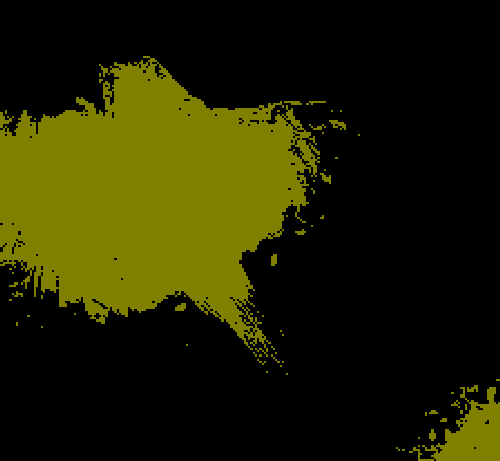
\includegraphics[width=0.18\linewidth, height=0.18\linewidth]{figures/ablation/withoutrfm/2008_001185_[2]} &
        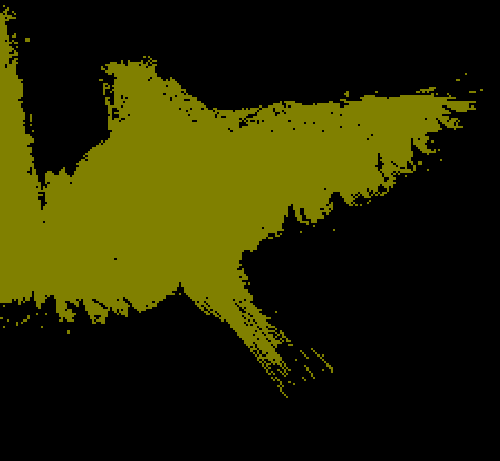
\includegraphics[width=0.18\linewidth, height=0.18\linewidth]{figures/ablation/withrfm/2008_001185_[2]} & \hspace{2pt}
        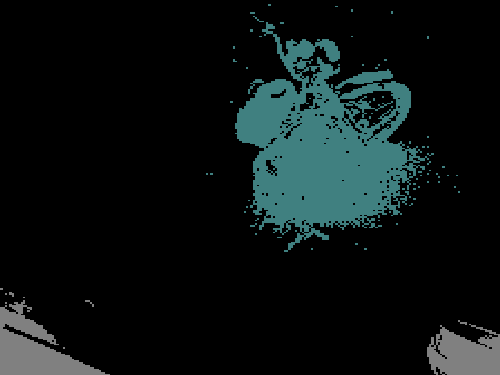
\includegraphics[width=0.18\linewidth, height=0.18\linewidth]{figures/ablation/withoutrfm/2008_007558_[6, 13]} &
        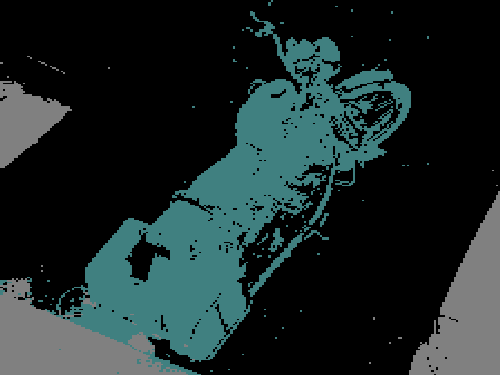
\includegraphics[width=0.18\linewidth, height=0.18\linewidth]{figures/ablation/withrfm/2008_007558_[6, 13]} \\
        [1mm]
        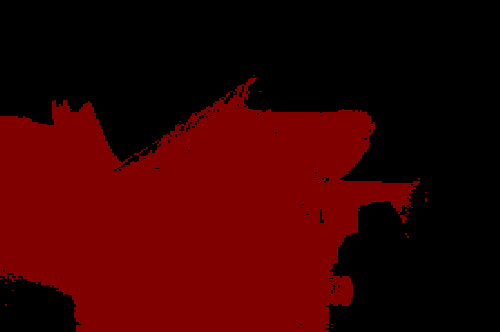
\includegraphics[width=0.18\linewidth, height=0.18\linewidth]{figures/ablation/withoutrfm/2011_001753_[0]} &
        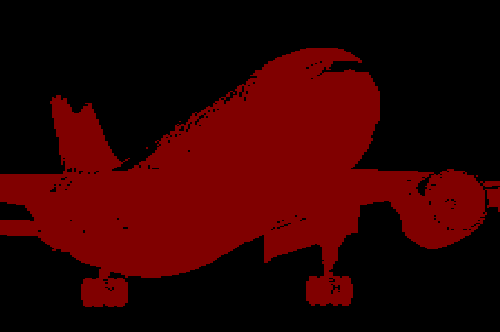
\includegraphics[width=0.18\linewidth, height=0.18\linewidth]{figures/ablation/withrfm/2011_001753_[0]} & \hspace{2pt}
        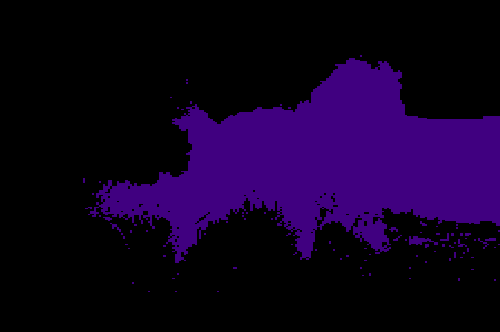
\includegraphics[width=0.18\linewidth, height=0.18\linewidth]{figures/ablation/withoutrfm/2011_002398_[11]} &
        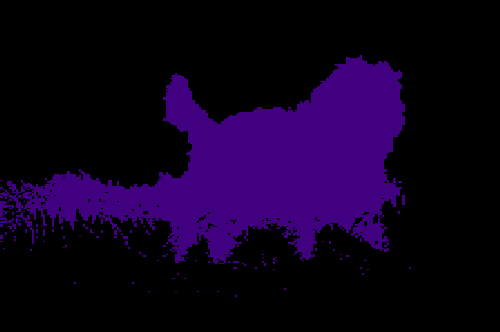
\includegraphics[width=0.18\linewidth, height=0.18\linewidth]{figures/ablation/withrfm/2011_002398_[11]} \\
        [1mm]
        
\includegraphics[width=0.18\linewidth, height=0.18\linewidth]{figures/ablation/withoutrfm/2007_009807_[12]} &
        
\includegraphics[width=0.18\linewidth, height=0.18\linewidth]{figures/ablation/withrfm/2007_009807_[12]} & \hspace{2pt}
        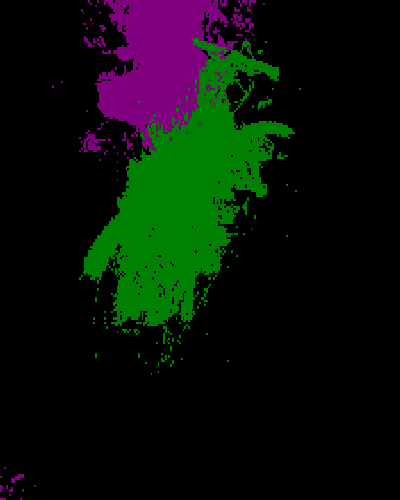
\includegraphics[width=0.18\linewidth, height=0.18\linewidth]{figures/ablation/withoutrfm/2010_003912_[1, 4]} &
        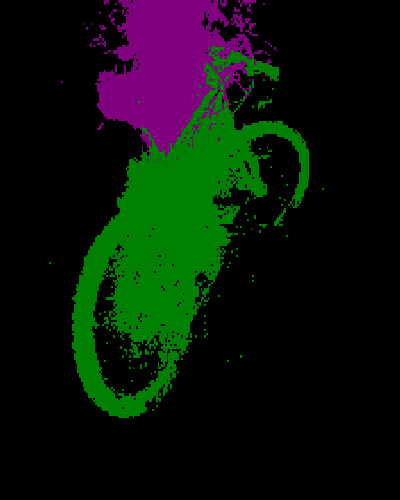
\includegraphics[width=0.18\linewidth, height=0.18\linewidth]{figures/ablation/withrfm/2010_003912_[1, 4]} \\
        [1mm]
        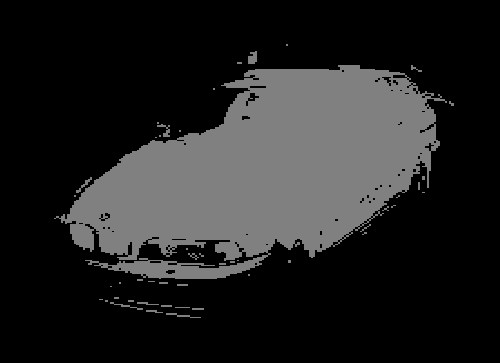
\includegraphics[width=0.18\linewidth, height=0.18\linewidth]{figures/ablation/withoutrfm/2010_003276_[6]} &
        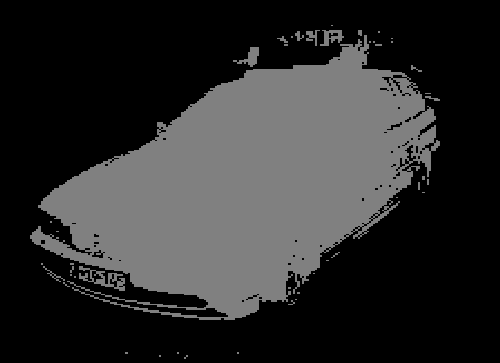
\includegraphics[width=0.18\linewidth, height=0.18\linewidth]{figures/ablation/withrfm/2010_003276_[6]} & \hspace{2pt}
        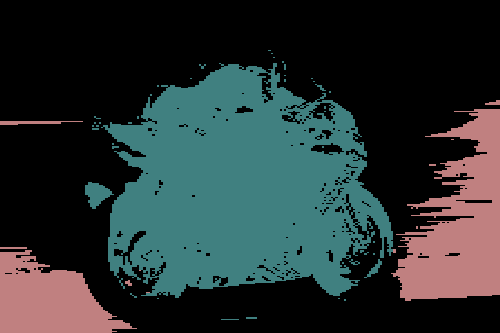
\includegraphics[width=0.18\linewidth, height=0.18\linewidth]{figures/ablation/withoutrfm/2009_000074_[13, 14]} &
        
\includegraphics[width=0.18\linewidth, height=0.18\linewidth]{figures/ablation/withrfm/2009_000074_[13, 14]} \\
      \end{tabular}
  }

  \caption{Qualitative ablation on the Pascal VOC dataset showing the effect of the Refinement Module (RFM) \cite{wsss_frozen_clip} using our method. Each pair compares pseudo-labels generated without (left) and with (right) RFM. The RFM enhances boundary precision and recovers missing object regions, leading to more complete and accurate segmentation masks.}
  \label{fig:qualitative_ablation}
\end{figure}

However, in some cases—most notably for the person class—the initial CAMs exhibit high confidence in background regions, which RFM further propagates during affinity-based refinement. This leads to over-segmentation and explains the slight quantitative drop observed for the person category in Table~\ref{tab:ablation_rfm_comparison}. Despite this limitation, RFM generally enhances semantic completeness and boundary precision, validating its role in improving spatial consistency under weak supervision.

Overall, the ablation study confirms that the RFM effectively enhances segmentation quality by refining initial CAMs using affinity information and contextual cues, particularly for classes that are underrepresented or have complex shapes. These results establish a strong baseline for subsequent experiments and highlight the importance of the RFM in improving both boundary delineation and class-specific performance.
